\documentclass{article}
\usepackage{amsmath}
\usepackage{parskip}
\usepackage{fullpage}
\usepackage{graphicx}
\usepackage{pgfplots}
\usepackage{neuralnetwork}

\title{Deep Learning}
\author{Paolo Bettelini}
\date{}

\graphicspath{ {Resources/} }

\begin{document}

\maketitle
\tableofcontents
\pagebreak

\section{Types of neurons}

\subsection{Brain neurons}

\begin{center}
    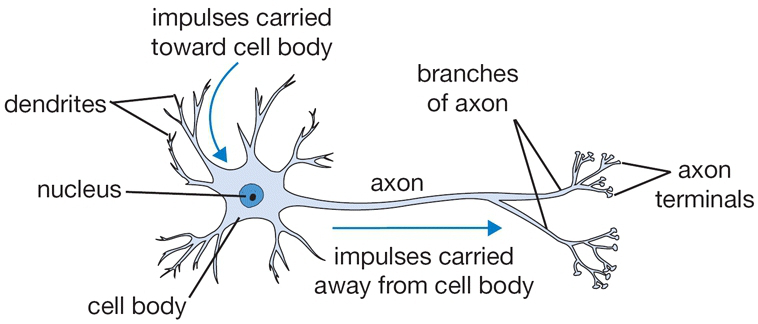
\includegraphics[scale=0.5]{neuron}
\end{center}

\subsection{Linear neurons}

% lecture 1.3

A linear neuron is very simple and computationally limited in what it can do.

\[
    y=b+\sum_{i} x_i w_i
\]

The output \(y\) is given by the bias \(b\) plus the sum of all the input connections \(x_i\) multiplied by their weight \(w_i\).

\subsection{Binary threshold neurons}

Binary threshold neurons output a \(1\) or a \(0\) depending on its weighted value.

Given a threshold \(\theta=-b\)
\begin{align*}    
    z&=b+\sum_{i} x_i w_i \\
    y&=\begin{cases}
        1 \text{ if } z\ge 0 \\
        0 \text{ otherwise}
    \end{cases}
\end{align*}

\subsection{Rectified Linear Neurons or Linear threshold neurons}

They compute a linear weighted sum of their inputs. \\
The output is a non-linear function of the total input.

Given a threshold \(\theta=-b\)
\begin{align*}    
    z&=b+\sum_{i} x_i w_i \\
    y&=\begin{cases}
        z \text{ if } z > 0 \\
        0 \text{ otherwise}
    \end{cases}
\end{align*}

\begin{center}
	\begin{tikzpicture}
		\begin{axis}[
            scale=0.75,
			xmin=-3,
			xmax=3,
			ymin=-3,
			ymax=3,
			xlabel={\(x\)},
			ylabel={\(y\)},
			scale only axis,
			axis lines=middle
		]
        \addplot[blue, ultra thick, domain=-3:0] {0};
        \addplot[blue, ultra thick, domain=0:2.5] {x};
		\end{axis}
	\end{tikzpicture}
\end{center}

\subsection{Sigmoid neurons}

They give a real-valued output that is a smooth and bounded function of their total input.

The logistic function is often used.

Given a threshold \(\theta=-b\)
\begin{align*}    
    z&=b+\sum_{i} x_i w_i \\
    y&=\frac{1}{1+e^{-z}}
\end{align*}

\begin{center}
	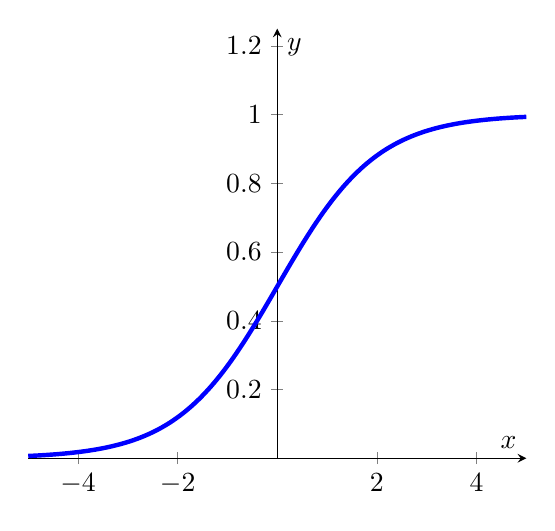
\begin{tikzpicture}
		\begin{axis}[
            scale=0.75,
			xmin=-5,
			xmax=5,
			ymin=0,
			ymax=1.25,
			xlabel={\(x\)},
			ylabel={\(y\)},
			scale only axis,
            smooth,
            samples=50,
			axis lines=middle
		]
        \addplot[blue, ultra thick, domain=-5:5] {1/(1+e^(-x))};
		\end{axis}
	\end{tikzpicture}
\end{center}

This function has smooth derivatives that change continuously. \\
This characteristic makes the learning process easier.

\pagebreak

% lecture 1.5

\section{Types of learning}

\subsection{Supervised learning}
Each training consists of making the network guess the target output \(t\) for a certain input \(x\), given the difference between the correct target and the guess we tweak the network.

There are two type of supervised learning

\subsubsection{Regression}
The target output is a numeric value of a vector of values. \\
To describe the error we can compute the square difference between the target output \(t\) and the actual output \(y\) of the module. \\
Often the value \(\frac{1}{2}{(t-y)}^2\) is used. The \(\frac{1}{2}\) coefficient is there to cancel the \(2\) out when differentiation is applied.

\subsubsection{Classification}
The target output is a class or label. Usually either \(1\) or \(0\).
There could also be multiple labels.
[\ldots]

\subsection{Reinforcement learning}
The output is an action of a sequence of actions to maximize the sum of rewards.

\subsection{Unsupervised learning}
[\ldots]

\pagebreak

% lecture 2.1

\section{Types of network architecture}

\subsection{Feed-forward neural network}

\begin{center}
    \begin{neuralnetwork}[height=4]
        \inputlayer[count=3, bias=false, title=Input\\units]
        \hiddenlayer[count=4, bias=false, title=Hidden\\units] \linklayers{}
        \outputlayer[count=2, title=Output\\units] \linklayers{}
    \end{neuralnetwork}
\end{center}

\subsection{Recurrent network}

\subsection{Symmetrically connected network}

\end{document}